%; whizzy chapter
% -initex iniptex -latex platex -format platex -bibtex jbibtex -fmt fmt
% 以上 whizzytex を使用する場合の設定。


%     Tokyo Debian Meeting resources
%     Copyright (C) 2009 Junichi Uekawa

%     This program is free software; you can redistribute it and/or modify
%     it under the terms of the GNU General Public License as published by
%     the Free Software Foundation; either version 2 of the License, or
%     (at your option) any later version.

%     This program is distributed in the hope that it will be useful,
%     but WITHOUT ANY WARRANTY; without even the implied warranty of
%     MERCHANTABILITY or FITNESS FOR A PARTICULAR PURPOSE.  See the
%     GNU General Public License for more details.

%     You should have received a copy of the GNU General Public License
%     along with this program; if not, write to the Free Software
%     Foundation, Inc., 51 Franklin St, Fifth Floor, Boston, MA  02110-1301 USA

%  preview (shell-command (concat "evince " (replace-regexp-in-string "tex$" "pdf"(buffer-file-name)) "&"))
% 画像ファイルを処理するためにはebbを利用してboundingboxを作成。
%(shell-command "cd image200905; ebb *.png")

%%ここからヘッダ開始。

\documentclass[mingoth,a4paper]{jsarticle}
\usepackage{monthlyreport}

% 日付を定義する、毎月変わります。
% date --date 'third saturday'
\newcommand{\debmtgyear}{2009}
\newcommand{\debmtgmonth}{5}
\newcommand{\debmtgdate}{16}
\newcommand{\debmtgnumber}{52}

\begin{document}

\begin{titlepage}
\thispagestyle{empty}

% タイトルページ:編集必要な部分は最初のマクロに飛ばすこと

\vspace*{-2cm}
第\debmtgnumber{}回 東京エリア Debian 勉強会資料

\hspace*{-2.4cm}
\includegraphics[width=210mm]{image200801/2008title.eps}\\
\hfill{}\debmtgyear{}年\debmtgmonth{}月\debmtgdate{}日

\end{titlepage}

\dancersection{Introduction}{上川 純一}

\begin{multicols}{2}
 
 
 今月のDebian勉強会へようこそ。これからDebianの世界にあしを踏み入れると
 いう方も、すでにどっぷりとつかっているという方も、月に一回Debianについ
 て語りませんか?

 Debian勉強会の目的は下記です。

 \begin{itemize}
 \item \underline{Debian Developer} (開発者)の育成。
 \item 日本語での「\underline{開発に関する情報}」を整理してまとめ、アップデートする。
 \item \underline{場}の提供。
 \begin{itemize}
  \item 普段ばらばらな場所にいる人々が face-to-face で出会える場を提供
	する。
  \item Debian のためになることを語る場を提供する。
  \item Debianについて語る場を提供する。
 \end{itemize}
 \end{itemize}		

 Debianの勉強会ということで究極的には参加者全員がDebian Packageをがりがり
 と作るスーパーハッカーになった姿を妄想しています。情報の共有・活用を通し
 て Debianの今後の能動的な展開への土台として、「場」としての空間を提供す
 るのが目的です。

 2009年の計画は仮です。

 \begin{enumerate}
  \item 新年の企画 (アンサンブル荻窪開催)
  \item OSC Tokyo
  \item VAIO P インストール記録、
	カーネル読書会 ディストリビューション大集合(小林さん)(東京大学?)
  \item Git Handson (岩松)(あんさんぶる荻窪?)
  \item 家Debianサーバ vs 職場のネットワーク(千代田区都立図書館?\footnote{\url{http://www.library.chiyoda.tokyo.jp/}})
  \item Asterisk (東京大学?)
  \item スペインにて開催
  \item Debconf報告会
  \item OSC Fall?
  \item udev + HAL(岩松さん)
  \item 3D graphics 開発(藤沢さん) 
  \item Debian サーバ+VMware + 各種OS、
	他の仮想化ツール(vserver etc.)、
	忘年会
 \end{enumerate}

 会場候補としては下記があります:

 \begin{itemize}
  \item 大学
  \item 恵比寿SGIホール
  \item Googleオフィス
  \item 公民館(あんさんぶる荻窪等)
  \item 都立会議室(無線LAN)
  \item 健保の施設
 \end{itemize}

\end{multicols}


\newpage

\begin{minipage}[b]{0.2\hsize}
 \definecolor{titleback}{gray}{0.9}
 \colorbox{titleback}{\rotatebox{90}{\fontsize{80}{80} {\gt デビアン勉強会} }}
\end{minipage}
\begin{minipage}[b]{0.8\hsize}
\hrule
\vspace{2mm}
\hrule

% set depth to 1 if too many text, 2 if there's less
\setcounter{tocdepth}{1}
\tableofcontents
\vspace{2mm}
\hrule
\end{minipage}

\dancersection{事前課題}{上川 純一}

事前課題は:

DDTSS
でいくつか(2個以上)Debianパッケージの説明文を翻訳してみて、2個レビューし
てみてください。その上で次の内容について説明してください:

\begin{enumerate}
 \item 適用した主要な方法
 \item 発見した課題
 \item 提案する理想像(ツールとか)、共有したい情報
\end{enumerate}

この課題に対して提出いただいた内容は以下です。

\begin{multicols}{2}
%; whizzy-master ../debianmeetingresume200905.tex
% $B0J>e$N@_Dj$r$7$F$$$k$?$a!"$3$N%U%!%$%k$G(B M-x whizzytex $B$9$k$H!"(Bwhizzytex$B$,MxMQ$G$-$^$9!#(B

\begin{prework}{$B>e@n=c0l(B}

\preworksection{$BE,MQ$7$?<gMW$JJ}K!(B}

DDTSS $B$r%V%i%&%6$GD/$a$F!"K]Lu$r%l%S%e!<$7$F$_$^$7$?!#(B
$B%Q%C%1!<%8$N(Bdescription$B$@$1$GJ,$+$i$J$$ItJ,$K$D$$$F$O%P%0%l%]!<%H$r$7$^(B
$B$7$?!#(B
$BITL@E@$O(B debian-doc@jp $B%a!<%j%s%0%j%9%H$K<ALd$H$7$FEj9F$7$^$7$?!#(B

\preworksection{$BH/8+$7$?2]Bj(B}

$B%l%S%e!<$r$7$FJ,$+$C$?$3$H$G$9$,!"K]Lu$N:n6H$GC18l$NK]Lu$^$G$O$G$-$F$$$k(B
$B$N$G$9$,!"J8>OA4BN$H$7$F78$j<u$1$,$*$+$7$/!"0UL#$,DL$C$F$$$J$$$b$N$,$"$j$^$7$?!#(B
$B$^$?!"1Q8l$N6gFIE@$r$=$N$^$^F|K\8l$N6gFIE@$KCV$-49$($F$*$j!"$=$N$^$^$G$OF|K\8l$H$7$F(B
$BJ8>O$,D9$9$.$k$b$N$b$"$j$^$7$?!#K]Lu:n6H$rD>Lu:n6H$H$9$k$HFI$_$K$/$$(B
Description$B$,$G$-$"$,$C$F$7$^$&$H;W$o$l$^$9!#(B

\preworksection{$BDs0F$9$kM}A[A|(B($B%D!<%k$H$+(B)$B!"6&M-$7$?$$>pJs(B}

\begin{itemize}
 \item Description $B$KBP$7$F$9$G$K%P%0%l%]!<%H$,Ej9F$5$l$F$$$k$+$I$&$+$N(B
       $B%A%'%C%/$9$k%D!<%k!#(B

 \item $BMQ8l=8$K$9$G$K7G:\$5$l$F$$$kMQ8l$r4JC1$K%&%'%V%V%i%&%6$+$i%A%'%C%/(B
       $B$G$-$k(Bgreasemonkey $B!#(B

 \item DDTSS $B$G9T$C$?%l%S%e!<!&%3%a%s%H$J$I$,(B debian-doc@jp $B%a!<%j%s%0%j(B
       $B%9%H$KH?1G$9$k$3$H!#(B
\end{itemize}

\end{prework}

\begin{prework}{$B$^$($@$3$&$X$$(B}
\preworksection{$BE,MQ$7$?<gMW$JJ}K!(B}
$B;vA02]Bj$^$G<j$,2s$i$:$8$^$$!#$@$1$@$H7]$,$J$$$N$G!"8=:_M'?M$H?J$a$F$$$k(B
 CouchDB$B$N(BWeb$B%5%$%H$NK]Lu$K$D$$$FOC$7$^$9!#(B
\begin{enumerate}
 \item CouchDB$B$N(BWeb$B%5%$%H$r(BGoogle Docs$B$G$^$k$4$H<h$j9~$`!##1%Z!<%8$K$D$-!"(B
       $BK]Lu<T$O8BDj!#B>$O::FI$7!"0lJ8$:$DK]Lu$9$k!#D>Lu$G$O$J$/!"F|K\8l(B
       $B$H$7$F$o$+$j$d$9$$J8>O$r=E;k!#(B
 \item Web$B%5%$%H!"(BWiki$B$r$"$kDxEY$NHfN($^$GK]Lu$r?J$a$k!#(B
 \item CouchDB$B$N3+H/<T8~$1$N(BML$B$K8x3+$7$?$$;]$rAjCL$9$k!#(B
 \item Debian$B$N(BCouchDB$B$N%Q%C%1!<%8%a%s%F%J$G$b$"$k!"3+H/<T$+$i(Bpo4a$B$r;H$&(B
       $B$3$H!"B>$K$b$$$m$$$m2]Bj!J%7%9%F%`4IM}!"%"%C%W%m!<%I$NJ}K!!"K]Lu(B
       $B$NDDIe2=$J$I!K$,$"$k$1$I$=$l$r9MN8$7$J$$$H$$$1$J$$$h$H!"%"%I%P%$(B
       $B%9$r$b$i$&!#(B
 \item PO$B7A<0$G%Q%C%AEj$2$FH?1G<+BN$O$*4j$$$7!"99?7$O$J$s$i$+$N<jCJ$G3N(B
       $BG'$7$F?o;~K]Lu$7$F$$$/;]$rEA$($k!#(B
 \item $B:#8e$NJ}?K$r$I$&$9$k$+$rM'?M$HAjCL$7$F!":#%3%3!#(B
\end{enumerate}

\preworksection{$BH/8+$7$?2]Bj(B}
Web$B%5%$%H$O(BXHTML$B$K$J$C$F$$$J$$$N$G!"$^$:JQ49$9$k$H$3$m$+$i;O$a$J$$$H$$$1(B
 $B$J$$$3$H$H!"(BWiki$B$O99?7$,IQHK$K$"$j$9$.$@$+$i!"BP>]$+$i30$7$?J}$,NI$$$h(B
 $B$M!"$HM'?M$HAjCL$7$?$H$3$m!#K]Lu$,$=$b$=$b$d$j$?$$$3$H$G$O$J$+$C$?$N$G!#(B

\preworksection{$BDs0F$9$kM}A[A|(B($B%D!<%k$H$+(B)$B!"6&M-$7$?$$>pJs(B}
$B:G=i$NK]Lu$@$19T$C$?$i!"8e$O<jN%$l$9$k!JC/$+$K0z$-7Q$0!K$N$,M}A[$G$O$"$k(B
 $B$b$N$N!"6(NO<T$rA}$d$5$J$$$H$$$1$J$$!#$=$b$=$b(BDebian$B%Q%C%1!<%8$K$J$C$F(B
 $B$$$k$N$G!"%=!<%9%Q%C%1!<%8$K4^$^$l$k%I%-%e%a%s%H$J$i!"(BDebian-doc$B$GK]Lu(B
 $B$7$F!"$=$C$A7PM3$G%"%C%W%9%H%j!<%`$KH?1G$7$F$b$i$&!"$H$$$&$N$b<j$@$J$H(B
 $B$$$&$3$H$r8!F$Cf!#(B
\end{prework}

\begin{prework}{$B$"$1$I(B}

$B@bL@J8$rK]Lu$7$?%Q%C%1!<%8(B
libvolpack1	$B%l%s%@%j%s%0%i%$%V%i%j(B
libvolpack1-dev	$B%l%s%@%j%s%0%i%$%V%i%j(B
nagios3		$B%7%9%F%`4F;k(B/$B4IM}%D!<%k(B
nagios3-doc	$B%7%9%F%`4F;k(B/$B4IM}%D!<%k$NJ8=q(B
cwcp		$B%b!<%k%9?.9fN}=,%=%U%H(B
dnswalk		DNS$B%A%'%C%/%D!<%k(B
slapd		LDAP$B%5!<%P(B
pingpong	$B%"%^%A%e%"L5@~MQ(B convers $B%5!<%P(B
sugar-presence-service	OLPC$BMQ%=%U%H(B
amap-align	DNA$B2r@O%D!<%k(B
loki		DNA$B2r@O%D!<%k(B
xastir		DNA$B2r@O%D!<%k(B
biosquid	DNA$B2r@O%D!<%k(B
boxshade	DNA$B2r@O%D!<%k(B
dialign		DNA$B2r@O%D!<%k(B
dialign-t	DNA$B2r@O%D!<%k(B
probcon		DNA$B2r@O%D!<%k(B

$B!A%l%S%e!<$3$3$+$i!A(B
$B%l%S%e!<(B 1
$B%Q%C%1!<%8(B: libvolpack1

Short description
$B86J8(B: fast volume rendering library
$BLuJ8(B: $B9bB.$JBgNL%l%s%@%j%s%0%i%$%V%i%j(B

Long description
$B86J8(B:
VolPack is a software library for fast, high-quality volume rendering with
this features:
 * Renders data sampled on a regular, three-dimensional grid.
 * Supports user-specified transfer functions for both opacity and color.
 * Provides a shading model with directional light sources, multiple material
   types with different reflective properties, depth cueing, and shadows.
 * Produces color (24 bits/pixel) or grayscale (8 bits/pixel) renderings,
   with or without an alpha channel.
 * Supports arbitrary affine view transformations.
 * Supports a flexible data format that allows an arbitrary C structure to be
   associated with each voxel.
$BLuJ8(B:
VolPack $B$O9bIJ<A$G9bB.$JBgNL$N%l%s%@%j%s%0$r9T$&%=%U%H%&%'%"%i%$%V%i%j$G!"(B
$B<!$NMM$JFCD'$r;}$C$F$$$^$9(B:
 * $B@55,2=$5$l$?%5%s%W%k%G!<%?$r(B 3 $B<!85%0%j%C%I$KI=<((B
 * $BITF)L@$H%+%i!<N>J}$N%f!<%6Dj5A$NJQ494X?t$r%5%]!<%H(B
 * $BJ}8~;XDj$5$l$?8w8;$K$h$k1"1FIU$-%b%G%k!"0c$&H?<MFC@-$r;}$C$?J#?t$NAG:`%?(B
   $B%$%W!"G;C8!"5Z$S1F$rDs6!(B
 * $B%"%k%U%!%A%c%M%k$NM-$j!"L5$7$N(B (24 $B%S%C%H(B/$B2hAG$N(B) $B%+%i!<$^$?$O(B (8 $B%S%C%H(B
   /$B2hAG$N(B) $B%0%l!<%9%1!<%9$G$NIA2h$N@8@.(B
 * $BG$0U$N;kE@$N%"%U%#%sJQ49$r%5%]!<%H(B
 * $BG$0U$N(B C $B8@8lE*$J9=B$$r%\%/%;%k(B (3 $B<!853J;R>e$N:G>.N)J}BN!"(B2 $B<!85$G$N(B
   $B%T%/%;%k(B) $B$X7k$S$D$1$k;v$,=PMh$k=@Fp$J%G!<%?%U%)!<%^%C%H$N%5%]!<%H(B

$B%l%S%e!<(B 2
$B%Q%C%1!<%8(B: amap-align

Short description
$B86J8(B: Protein multiple alignment by sequence annealing
$BLuJ8(B: $B%7!<%/%(%s%9%"%K!<%j%s%0$K$h$kCAGr<A$N%^%k%A%W%k%"%i%$%a%s%H(B ($BB?=EG[Ns@0Ns(B)

Long description
$B86J8(B:
AMAP is a command line tool to perform multiple alignment of peptidic
sequences. It utilizes posterior decoding, and a sequence-annealing
alignment, instead of the traditional progressive alignment method. It
is the only alignment program that allows to control the sensitivity /
specificity tradeoff.  It is based on the ProbCons source code, but
uses alignment metric accuracy and eliminates the consistency
transformation.
.
 Homepage: http://bio.math.berkeley.edu/amap/
$BLuJ8(B:
AMAP $B$O%Z%W%A%IG[Ns$N%^%k%A%W%k%"%i%$%a%s%H(B ($BB?=EG[Ns@0Ns(B) $B$r9T$&%3%^%s%I(B
$B%i%$%s%D!<%k$G$9!#;v8e2rFI$KMxMQ$5$l!"EAE}E*$J%W%m%0%l%C%7%V%"%i%$%a%s%H(B
$BK!$NBe$o$j$K%7!<%/%(%s%9%"%K!<%j%s%0$N@0Ns$r9T$$$^$9!#46EY(B \& $BFC0[@-$N(B
$B%H%l!<%I%*%U$r%3%s%H%m!<%k=PMh$kM#0l$N%"%i%$%a%s%H(B ($B@0Ns(B) $B%W%m%0%i%`$G$9!#(B
ProbCons $B$N%=!<%9%3!<%I$r85$K$7$F!"@:L)B,Dj%"%i%$%a%s%H(B ($B@0Ns(B) $B$H%3%s%7(B
$B%9%F%s%7!<%H%i%s%9%U%)!<%a!<%7%g%s(B ($B0l4S@-JQ2=(B) $B$N=|5n$rMxMQ$7$F$$$^$9!#(B
.
 Homepage: http://bio.math.berkeley.edu/amap/

$B!A%l%S%e!<$3$3$^$G!A(B

1$B!#E,MQ$7$?<gMW$JJ}K!(B
$B<jF~NO$H%M%C%H>e$N1QOB<-E5!"I,MW$K1~$8$F(B Google$B!"(Bwikipedia$B!"$=$NB>@lLg%5%$%H$r;2>H(B

2$B!#H/8+$7$?2]Bj(B
DNA$B2r@O%D!<%k$,B?$/$"$j!"@lLgMQ8l$,$^$A$^$A$G(B
$B$=$l$NE}0l<c$7$/$O6&DL2=$,I,MW$@$H;W$$$^$7$?!#(B

3$B!#Ds0F$9$kM}A[A|(B($B%D!<%k$H$+(B)
$B@lLgMQ8l$K$D$$$F$O<-=q%Z!<%8$rMQ0U$9$k$+!"4p=`$K$9$k@lLgMQ8l$N%5%$%H$r7h$a$k$N$,NI$$$+$H;W$$$^$9!#(B

$B!&6&M-$7$?$$>pJs$r@bL@(B
Debian $B%Q%C%1!<%8$K$O?tB?$/$N(B DNA $B2r@O%D!<%k$,$"$C$F!"@lLgMQ8l$NK]Lu$K$"$?$C$FCm0U?<$/:n6H$9$kI,MW$,$"$k$H;W$$$^$9!#(B
DNA $B2r@O$K$D$$$FM=HwCN<1$H$7$F2<5-%5%$%H$,;29M$K$J$k$+$H;W$$$^$9!#(B
$B%?%s%Q%/<A!?3K;@$N%"%i%$%a%s%H2r@O(B 
http://www.icot.or.jp/ARCHIVE/Museum/SOFTWARE/GIP/gene\_alignment.html
$B"(J8;z%3!<%I$,(B ISO-2022-JP $B$J$N$K%(%s%3!<%I>pJs$O(B Shift-JIS $B$K$J$C$F$$$^$9!#(B

Debian JP $BJ8=q:n@.$N;X?K(B $B$K$D$$$F(B DDTSS for ja $B$K%j%s%/$,$"$C$?J}$,NI$$$+$H;W$$$^$9!#(B

\end{prework}

\begin{prework}{$BF|HfLn(B $B7<(B}
DDTSS$B$G(Bocaml$B$H(Blibperl4caml-ocaml$B$N(BDescription$B$rK]Lu$7$F$_$^$7$?!#(B
$B%l%S%e!<$O(Bnasm$B$H(Blibobjc2$B$r$d$C$F$_$^$7$?!#(B

\preworksection{$BE,MQ$7$?<gMW$JJ}K!(B}

DDTSS$B$N(BWeb$B%$%s%?!<%U%'!<%9$+$iK]Lu$H%l%S%e!<$r9T$J$C$F$_$^$7$?!#(B

\preworksection{$BH/8+$7$?2]Bj(B}

$B<+J,$,K]Lu$r9T$J$C$?FbMF$,99?7$5$l$?$H$-$d(B
$B%3%a%s%H$,IU$$$?$H$-$K!":F$S8+$K$$$+$J$$$H99?7$rCN$k$3$H$,(B
$B$G$-$J$$$N$,5$$K$J$j$^$7$?!#(B

\preworksection{$BDs0F$9$kM}A[A|(B($B%D!<%k$H$+(B)$B!"6&M-$7$?$$>pJs(B}

$BK]Lu$7$??M$d%l%S%e!<$7$??M$K99?7$rDLCN$9$k5!G=$H(B
$B$=$l$r%3%s%H%m!<%k$9$k5!G=$,M_$7$$$G$9!#(B
\end{prework}

\begin{prework}{$B>.@n(B $B?-0lO:(B}
 $B0J2<!$$d$C$F$_$?46A[$J$I!%(B
 \preworksection{$BEPO?(B}
 $B$^$:EPO?;~$N(B Alias $B$H8@$&$N$,D>46$G$o$+$j$^$;$s$G$7$?!%(B
 \preworksection{$BK]Lu(B}
 $BK]Lu$O0J2<$N#2$D$N%Q%C%1!<%8$K$D$$$F$d$C$F$_$^$7$?!%(B
 \begin{itemize}
  \item wgerman-medical
  \item libbio-ruby
 \end{itemize}
 $B;W$C$?$N$O!$$$$-$J$jA4$F$rLu$5$J$1$l$P$J$i$J$$$N$O?I$$$s$8$c$J$$$+$H8@(B
 $B$&$3$H!%>/$7$:$DK]Lu$G$-$?$j!$$b$7$/$OESCf7k2L$rJ]B8$G$-$k$?J}$,$$$$$s(B
 $B$8$c$J$$$+$H;W$$$^$7$?!%(B

 $B$"$H$O!$:G=i$K$I$&2?$r$9$l$P$$$$$N$+$,$o$+$j$K$/$H8@$&$3$H!%(B
 $B$o$+$C$?Ev$?$jA0$J$N$+$bCN$l$^$;$s$,!$I}9-$/6(NO<T$r5a$a$k$N$J$i!$2?$+(B
 $B$7$i>pJs(B(HowTo$B$H$+!)(B)$B$"$C$?J}$,$$$$5$$,$7$^$9!%(B
 \preworksection{$B%l%S%e!<(B}
 $B$$$-$J$j(B 'Accept as is' $B$H=q$+$l$k$N$,I]$+$C$?!%$A$c$s$H!$(B
 ``'Accept as is' means you agree with this translation.''
 $B$H=q$+$l$F$O$$$k$s$G$9$,!$$I$&$K$b!V$($C!$$$$$$N$+!)!W$H8@$&;W$$$,H4$1(B
 $B$-$l$^$;$s$G$7$?!%$N$G!$%l%S%e!<$O8+$?$@$1$G$9!%(B

 $B$G!$(Bmultimail $B$r8+$?$H$-$N46A[$G$9$,!$(Bdiff $B$r$b$&>/$7$o$+$j$d$9$/I=<($G(B
 $B$-$J$$$+$H;W$$$^$7$?!%(B
 $B$5$9$,$KA08e$K$"$k$H!$F,$NCf$G$$$m$$$mAH$_N)$F$J$$$HFI$a$J$$$N$G!$(B
 $B>e2<$K0[$J$kItJ,$@$1J8;zD9$rJ;$;$FI=<($G$-$?$j$9$k$H!$$o$+$j$d$9$$$+$J(B
 $B$H!%(B

 $B!V;W$C$?!W$P$+$j$N46A[$K$J$C$F$7$^$$$^$7$?$,!$$3$s$J46$8$G$7$?!%(B
\end{prework}

\begin{prework}{$B$d$^$@$?$/$^(B}

\preworksection{$BE,MQ$7$?<gMW$JJ}K!(B}

DDTSS $B$h$j86J8$HLuJ8$rF~<j$7$F!"K]Lu;Y1g%D!<%k(B OmegaT $B$^$?$O%F%-%9%H(B
$B%(%G%#%?$GK]Lu$7$^$7$?!#J#?t$N%*%s%i%$%sHG$N<-=q!"%Z!<%Q!<HG$N<-=q!"K]Lu(B
$B%=%U%H!"BP>]%=%U%H%&%'%"!"(BWeb $B8!:w!"=q@R$ND4::$rJ;MQ$7$^$7$?!#(B
$B%l%S%e!<0MMj$r(B debian-doc $B%a!<%j%s%0%j%9%H$KEj9F$7$^$7$?!#(B
$B>pJsDs6!0MMj$r(B YLUG $B%a!<%j%s%0%j%9%H$KEj9F$7$^$7$?!#(B

\preworksection{$BH/8+$7$?2]Bj(B}

Deiban JP $B4XO"$NK]Lu$N%7%9%F%`$H1?MQ$K$D$$$F$N>pJs<}=8$NFq0WEY$,9b$$(B
$B>uBV$G$7$?!#%I%-%e%a%s%H$,@0Hw$5$l$F$$$J$$>pJs$d!"?tG/4V%"%C%W%G!<%H$5$l$F(B
$B$$$J$$%Z!<%8$,$"$j$^$7$?!#(B

$BMW5a$5$l$kLu$NIJ<A$,ITL@$J$?$a!":n6H;~4V$d:n6H<j=g$N8+@Q$j$,:$Fq$G$7$?!#(B

$BLu$NIJ<A0BDj$KI,MW$J<9I.4p=`$N@0Hw>u67$,IT==J,$G$7$?!#(B

\preworksection{$BDs0F$9$kM}A[A|(B($B%D!<%k$H$+(B)$B!"6&M-$7$?$$>pJs(B}

\begin{itemize}
 \item $B:n6H<j=g%Z!<%8$N%"%C%W%G!<%H!#(B

 \item $B<9I.4p=`$HMQ8l=8$N%"%C%W%G!<%H!#(B

 \item $B<9I.4p=`E,9g%F%9%H%D!<%k$dK]Lu;Y1g%D!<%kMQ%i%$%V%i%j$NDs6!$,$G$-(B
       $B$k$H$&$l$7$$$G$7$g$&!#(B
\end{itemize}

\end{prework}

\begin{prework}{$B$d$^$M$R$G$-(B}

\preworksection{$BE,MQ$7$?<gMW$JJ}K!(B}

DDTSS $B$r%V%i%&%6$GD/$a$F!"K]Lu!u%l%S%e!<!D$7$?$h$&$J5-21$,Hy$+$K$"$j$^$9!#(B

\preworksection{$BH/8+$7$?2]Bj(B}

$B0l?M$@$H<d$7$9$.$k!#$H$$$&$N$O$5$F$*$-!"A4BNA|$H8=>u$NGD0.$,Fq$7$/!"0lBN$I$3$+$i$3$N;3$r(B
$BEP$l$P$$$$$N$+$h$/J,$+$i$J$$>uBV$@$C$?5-21$,!#(B

\preworksection{$BDs0F$9$kM}A[A|(B($B%D!<%k$H$+(B)$B!"6&M-$7$?$$>pJs(B}

\begin{itemize}
 \item $B8+$d$9$$%Z!<%89=@.$,M_$7$$!#AGKQ2a$.$F2?$,2?$d$iJ,$+$i$s$N$O4*J[!#$;$a$F(Bpo-debconf$B$N%Z!<%8(B(http://www.debian.org/international/l10n/po-debconf/ja)$B%l%Y%k$N$OM_$7$$!#(B
 \item $B!V0l%f!<%6$,FI$s$GM}2r$G$-$k!WJ8>O$r?4$,$1$k$3$H!#Ev$?$jA0$J$s$G$9$,!"Fq$7$$$N$G2~$a$F!J5U$K8@$&$H!"::FI$O%f!<%6$K$7$F$b$i$&;EAH$_$,M_$7$$$H$3$m$G$9!K!#(B
\end{itemize}

\end{prework}

\end{multicols}

% image200905/prework.tex 内部にテキストを追加してください。
%
%

\dancersection{最近のDebian関連のミーティング報告}{上川 純一}
\subsection{東京エリアDebian勉強会51回目報告}
% (query-replace-regexp "<.*?>" "")
% (query-replace-regexp "^[	 ]\+" "")

東京エリアDebian勉強会報告。
2009年4月18日土曜日に
東京エリアDebian勉強会の
第51回
をあんさんぶる荻窪にて開催しました。

今回の参加者は
中尾、北原、明渡、眞戸江、小川、
山本、 山田たくま 、高橋(masaka)、 前田耕平、 吉田@板橋、日比野、吉藤、でんすけ
藤澤りそう,上川x2
の16名でした。

まず、クイズ。

前田さんがjava policyを読んでみたので話をしました。
まだパッケージ作成には着手していないようなので今後パッケージ作成レポートが出てくるかな?

上川がocamlをつかってみたので報告。
Debian 上でocamlをつかったパッケージが意外とたくさんあるということで盛り上がりました。
しかしまだ十分入門できていないのでこれからかな。

その後、Debian開発のワークフローについてディスカッション。
事前課題を紹介していたら時間が尽きたので深い議論はなかった感じで。
いろいろと紹介されていたので面白かったのではないでしょうか。

宴会ははなの舞西荻窪店で。

%============================================================
%%% trivia quiz
\dancersection{Debian Trivia Quiz}{上川 純一}

ところで、みなさん Debian 関連の話題においついていますか?Debian関連の話
題はメーリングリストをよんでいると追跡できます。ただよんでいるだけではは
りあいがないので、理解度のテストをします。特に一人だけでは意味がわからな
いところもあるかも知れません。みんなで一緒に読んでみましょう。

今回の出題範囲は\url{debian-devel-announce@lists.debian.org} に投稿された
内容とDebian Project Newsからです。

\begin{multicols}{2}
 %; whizzy-master ../debianmeetingresume200905.tex
% $B0J>e$N@_Dj$r$7$F$$$k$?$a!"$3$N%U%!%$%k$G(B M-x whizzytex $B$9$k$H!"(Bwhizzytex$B$,MxMQ$G$-$^$9!#(B
%
% $B$A$J$_$K!"%/%$%:$OJL%V%i%s%A$G:n@.$7!"$N$A$K%^!<%8$7$^$9!#5U$K%^!<%8$7(B
% $B$J$$$h$&$K$7$^$7$g$&!#(B
% (shell-command "git checkout quiz-prepare")

\santaku
{}
{}
{}
{}
{}
\end{multicols}

% ===============================================================
\dancersection{Erlang コードをDebianパッケージにしてみた}{前田 耕平}
\index{erlang}
% ===============================================================

\subsection{入門のきっかけ}
Erlangというプログラミング言語があります。今回、これを勉強してみようと思っ
たのは、Erlangそのものがきっかけではなく、いつものように別のものがきっか
けです。今回は、CouchDBというApache
Incubator\footnote{\url{http://incubator.apache.org/}}にあった
\footnote{現在は、Apache Incubatorから卒業してApache Projectの一つになっ
ています。\url{http://couchdb.apache.org/}}、ドキュメント指向のデータベー
スを友人から教えてもらったのがきっかけでした。CouchDBがErlang と
JavaScriptで実装されている、というので、「Erlangって何だろう?」と興味を
持ちました。

\subsubsection{ちょっと脱線:CouchDBとは}
CouchDBの特徴には以下のものがあります。
\begin{itemize}
 \item ドキュメント指向
 \item スキーマレス
 \item RESTful
 \item JSON形式でデータをやりとり
\end{itemize}

RDBのように事前にしっかりとスキーマの定義を行っておく必要はなく、HTTP
PUTでデータ(=ドキュメント)を作成・更新し、GETでデータを取得し、DELETE
でデータを削除する、ちょっと変わったデータベースです。RDBを置き換えるも
のではないので、摘要範囲は正直まだよく分かりません。ですが、面白そうなの
で友人とこれを広めるべく、目下水面下で活動中です。

CouchDBのアーキテクチャについては、CouchDB Projectのホームページから転載
した、下記のシステム概念図をご覧下さい。これらの実装は主に Erlangによるものです。

また、CouchDBについては、水面下の活動の一環で翻訳なども行っているので、また別
の機会にお話できればと思います。


\subsubsection{閑話休題:Erlangの概要}
本題のErlangですが、CouchDBに興味を持ち、さらにその中身をどうなっている
のを知りたいと思ったのですが、Erlangという言語を知りません。関数型プログ
ラミングで、並列処理、分散処理、耐障害性を兼ね備えた、並行指向プログラミ
ングというのですが、そもそも文法がまったく分からないので、ソースコードだ
けを眺めて理解できるものではないな、ということから勉強を始めてみました。
また、並列処理、分散処理に興味を持っていたので、興味がうまい具合に重なっ
たのも、きっかけとなりました。

\subsubsubsection{Erlangの歴史}
Erlangは、Ericsson Computer Science Laboratoryで、分散化された環境、耐障
害、ある程度のリアルタイム性、無停止で稼働する、といった条件のシステムを
構築できるように設計されたプログラミング言語です。もともとは、エリクソン
の社内だけで使われていましたが、1998年にオープンソースとして公開されまし
た。ライセンスは、Erlang Public
License\footnote{\url{http://erlang.org/EPLICENSE}}で、Mozilla Public
Licenseの派生ライセンスです。関数型で並列指向のプログラミング言語という
ことですが、20年を超える歴史と、高度な信頼性が要求される通信機器の分野で
も実績があり、例えばエリクソンのAXD301\footnote{ATMスイッチ}などがあるそうで
す。

\subsubsubsection{仕様}
プログラミングErlangという書籍を一通り読んで、今2周目で実際に手を動かし
ている段階ですが、その中で興味を持った特徴を挙げます。

\begin{itemize}
 \item 評価できるものは全て式
 \item 変数の書き換えはできない
 \item 関数型プログラミング言語
 \item 並行処理(並行プログラミング)
\end{itemize}
自分には馴染みが薄いものばかりです。特に、「変数の書き換えはできない」な
んて、定数じゃないの?と思いました。詳しくは後述。

\subsubsubsection{Erlangによる最近の実装例}
Erlangで実装されているソフトウェアの例です。これらはdebパッケージになっ
ており、Lennyにも含まれています。
\begin{itemize}
 \item CouchDB
 \item ejabberd\footnote{\url{http://ejabberd.jabber.ru/}} twitterで使わ
       れているというIMサーバ
 \item YAWS(Yet another web
       server)\footnote{\url{http://yaws.hyber.org/}} Erlangで実装された
       Webサーバ
\end{itemize}

\subsubsubsection{Erlangの検証事例}
数年前から、一部では流行りらしいので、検証事例もちらほら出ています。
\begin{itemize}
 \item KLab株式会社による検証
       \begin{itemize}
	\item Erlang Performance \\
	      \url{http://lab.klab.org/wiki/Erlang_Performance}
	\item Erlang Process \\
	      \url{http://lab.klab.org/wiki/Erlang_Process}
       \end{itemize}     
 \item Erlang vs. Stackless python: a first benchmark \\
       \url{http://muharem.wordpress.com/2007/07/31/erlang-vs-stackless-python-a-first-benchmark/}
       \end{itemize}

一般的に普及していくのはまだこれからみたいな感じしますが、あまり使われて
いないうちに遊んでおこうと思います。

\subsection{環境を整える}
Debianでは数はまだ少ないもののErlangとErlangで書かれたソフトウェアのパッ
ケージがあります。
\begin{commandline}
$ apt-cache search erlang | wc -l
63
\end{commandline}

ちなみに、例として挙げたCouchDBやYAWSもdebパッケージになっています。

Erlangを使うために最低限必要なパッケージは次のerlang-baseパッケージです。
対話型ではなく、ソースコードを書くのにはemacsのErlang用のモードもあるの
で、それも一緒にインストールしておくと良いでしょう。

\begin{commandline}
$ sudo apt-get install erlang-base erlang-mode
\end{commandline}

ところで、erlang-baseパッケージではなく、erlangパッケージをインストールす
れば、erlangソースパッケージから分割されている関連パッケージも軒並みイン
ストールされるので便利かもしれませんが、この場合は依存関係も含めて関連す
るパッケージが90以上導入されます。状況に応じて適宜選択してください。

\begin{commandline}
$ sudo apt-get install erlang
\end{commandline}

\subsection{対話型で使ってみる}
対話型でErlangを使うには、erlコマンドを実行します。すると、Erlang
shell(Eshell)が起動します。

\begin{commandline}
$ erl
Erlang (BEAM) emulator version 5.6.5 [source] [64-bit] [smp:2] [async-threads:0] [kernel-poll:false]

Eshell V5.6.5  (abort with ^G)
1> 
\end{commandline}

``1$>$'' はプロンプトです。Eshellを終了するには、q().と入力するか、
\begin{commandline}
1> q().
ok
2> $
\end{commandline}

または、ctrl+ c, aと入力します。

\begin{commandline}
1>
BREAK: (a)bort (c)ontinue (p)roc info (i)nfo (l)oaded
       (v)ersion (k)ill (D)b-tables (d)istribution
a
$
\end{commandline}

では、変数を書き換えれない、という件の特徴をみてみます。
\begin{commandline}
1> A=10.
10
2> A=20.
** exception error: no match of right hand side value 20
\end{commandline}
見ての通り、エラーになってしまいました。Erlangの変数の書き換えはできな
い、単一代入変数なのです。もう一度代入の仕方を変えて見てみましょう。

\begin{commandline}
1> A1=1.
1
2> A2=2.
2
3> A3=A1+A2.
3
4> A3=3.
3
5> A3=A1+2. 
3
6> A3=A1+4.
** exception error: no match of right hand side value 5
7> A1=A2+A3. 
** exception error: no match of right hand side value 5
8> A1=A3-A2.
1
\end{commandline}

1,2,3のように未代入の変数に対しては値を再代入できますが、6,7のように一度
代入された変数に対しては違う値を代入しなおすことができないことが分かりま
す。しかし、4,5,8のように同じ値であれば再代入できるように見えます。
実は、4,5,8は変数を再代入しているわけではなく、代入済みの変数に対し、パ
ターン照合を行っているのです。

代入済みの変数のことを束縛済み変数、と言いますが、未束縛状態の変数に対
しては、イコールは値の代入を行いますが、束縛済みの変数に対してはパター
ン照合を行う、という訳です。

今までこんな仕様のプログラミング言語は見たことなかったのですが、プログラ
ミング言語ではなく、実は数学の代数であれば同じような考え方ができることが
分かります。例えば、$ x + y = 6, x - y = 2$という関数を考えてみます。こ
の状態では、x, yの代数はx=4, y=2以外の値にはなりません。単一代入変数は、
数学の代数と同じようなものと考えれば、良いのかもしれません。

\subsection{コンパイルしてみる}
次に、ソースコードからコンパイルして実行する方法について説明します。プロ
グラムを実行する方法は、次の3種類があります。
\begin{itemize}
 \item Eshellからコンパイルして実行する。
 \item シェルからコンパイルして実行する。
 \item escriptとして実行する。
\end{itemize}

例としてはやはり、Hello Worldを書いてみます。これは引数なしのプログラム
です。引数ありとなしではプログラム実行時に若干の違いが出てきます。
hello.erlというファイル名で次のプログラムを用意して下さい。

\begin{commandline}
-module(hello).
-export([start/0]).

start() ->
    io:format("Hello world on Erlang~n").
\end{commandline}

Erlangのプログラムはモジュールを基本単位とし、どの関数もモジュールに属す
 る構造になっています。コードを実行するには、まずモジュールをコンパイル
 しなければなりません。コンパイルしたモジュールは、拡張子
 beam\footnote{Bogdan's Erlang Abstract Machineの略。}という名前のファイ
 ルが生成されます。コンパイルには2つのやり方があります。

\subsubsection{Eshellからコンパイルする方法}
先ほどのhello.erlをEshellからコンパイルし、実行するには、次の手順です。

\begin{commandline}
1> c(hello).
{ok,hello}
2> he
heart    hello    
2> hello:start().
Hello world on Erlang
ok
3> 
\end{commandline}

c(hello).でコンパイルの実行を行います。c()の引数がmodule(hello)および、
プログラムファイル名hello.erlと一致することに注意してください。コンパイ
ルすると、hello.beamファイルが生成されます。これはErlang VM向けのバイナ
リコードです。

\begin{commandline}
$ ls -lrt hello.*
-rwx------ 1 user user   90 2009-05-14 01:35 hello.erl
-rw------- 1 user user  552 2009-05-14 01:35 hello.beam
$ file hello.beam 
hello.beam: Erlang BEAM file
\end{commandline}

\subsubsection{シェルからコンパイルする}
シェルからコンパイルする場合は、erlcコマンドを使います。

\begin{commandline}
$ erlc hello.erl
$ ls -lrt hello.*
-rwx------ 1 user user   90 2009-05-14 01:35 hello.erl
-rw------- 1 user user  708 2009-05-14 01:53 hello.beam
\end{commandline}

実行もシェルから行ってみます。

\begin{commandline}
$ erl -noshell -s hello start -s init stop
Hello world on Erlang
\end{commandline}

無事、実行できました。なお、各引数は次の意味があります。

\begin{itemize}
 \item -noshell \\
       対話型シェルなしでErlangを起動する。
 \item -hello start \\
       関数hello:start()を実行する。
 \item -init stop \\
       apply(hello, start, [])が完了すると\footnote{-s ...コマンドはapply
       文で評価される。1つのコマンドが完了すると次の-s ...コマンドが評価
       される。}、システムは関数init:stop()を評価する。
\end{itemize}

\subsubsection{escriptで実行する}
Erlangではescriptという仕組みもあり、これを使うとプログラムをコンパイル
せずにスクリプトとして直接実行できます。

関数hello:startをescriptとして実行するには、次のようにファイルを書き換え
ます。ファイル名は今回、hello.escとしましたが、コンパイルするときと違い、
任意の拡張子で問題ありません。
\begin{commandline}
#!/usr/bin/env escript

main(_) ->
    io:format("Hello world on Erlang~n").
\end{commandline}

これを実行権限をつけて実行してみます。
\begin{commandline}
$ chmod 700 hello.esc 
$ ./hello.esc 
Hello world on Erlang
\end{commandline}

\subsubsection{引数ありの関数をコンパイル、実行する}
今回の例は、引数なしでしたが、シェルで実行する場合のプログラムはどうやっ
て引数を渡せば良いのでしょうか。今度は引数ありのプログラムを試してみます。

フィボナッチ数列を計算する関数を書いてみました。まず、Eshellで引数を渡す場合です。
\begin{commandline}
-module(fib).
-export([fib/1]).

fib(0) -> 1;
fib(1) -> 1;
fib(N) ->
    fib(N-2) + fib(N-1).
\end{commandline}

実行するとこんな感じ。

\begin{commandline}
1> c(fib)
1> .
{ok,fib}
2> fib:fib(10).
89
3> fib:fib(20).
10946
4> fib:fib(30).
1346269
\end{commandline}

シェルから実行する場合は、書き方を変える必要があります。

\begin{commandline}
-module(fib1).
-export([main/1]).

main([A]) ->
    I = list_to_integer(atom_to_list(A)),
    F = fib(I),
    io:format("fibonacci ~w = ~w~n", [I, F]),
    init:stop().

fib(0) -> 1;
fib(1) -> 1;
fib(N) ->
    fib(N-2) + fib(N-1).
\end{commandline}

これをシェルでコンパイル、実行してみます。
\begin{commandline}
$ erlc fib1.erl
$ erl -noshell -s fib1 main 10 -s init stop
fibonacci 10 = 89
$ erl -noshell -s fib1 main 20 -s init stop
fibonacci 20 = 10946
$ erl -noshell -s fib1 main 30 -s init stop
fibonacci 30 = 1346269
\end{commandline}

\subsection{debパッケージにしてみる}
前述のとおり、Erlangはbeamファイルからコードをロードするか、escript
で実行する必要があります。Erlangのランタイムシステムは、コード自動ロード
機構を利用しています。現在のロードパスはEshellからcode:get\_path()確認す
ることができます。

\begin{commandline}
1> code:get_path().
[".","/usr/lib/erlang/lib/kernel-2.12.5/ebin",
 "/usr/lib/erlang/lib/stdlib-1.15.5/ebin",
 "/usr/lib/erlang/lib/xmerl-1.1.10/ebin",
 "/usr/lib/erlang/lib/webtool-0.8.3.2/ebin",
 "/usr/lib/erlang/lib/typer-0.1.5/ebin",
 "/usr/lib/erlang/lib/tv-2.1.4.2/ebin",
 "/usr/lib/erlang/lib/tools-2.6.2/ebin",
 "/usr/lib/erlang/lib/toolbar-1.3.0.1/ebin",
 "/usr/lib/erlang/lib/test_server-3.2.4/ebin",
 "/usr/lib/erlang/lib/syntax_tools-1.5.6/ebin",
 "/usr/lib/erlang/lib/ssl-3.10/ebin",
 "/usr/lib/erlang/lib/ssh-1.0.2/ebin",
 "/usr/lib/erlang/lib/snmp-4.12/ebin",
 "/usr/lib/erlang/lib/sasl-2.1.5.4/ebin",
 "/usr/lib/erlang/lib/runtime_tools-1.7.3/ebin",
 "/usr/lib/erlang/lib/public_key-0.1/ebin",
 "/usr/lib/erlang/lib/pman-2.6/ebin",
 "/usr/lib/erlang/lib/percept-0.7.3/ebin",
 "/usr/lib/erlang/lib/parsetools-1.4.5/ebin",
 "/usr/lib/erlang/lib/otp_mibs-1.0.4.1/ebin",
 "/usr/lib/erlang/lib/os_mon-2.1.8/ebin",
 "/usr/lib/erlang/lib/orber-3.6.10/ebin",
 "/usr/lib/erlang/lib/odbc-2.10.3/ebin",
 "/usr/lib/erlang/lib/observer-0.9.7.4/ebin",
 "/usr/lib/erlang/lib/mnesia-4.4.7/ebin",
 "/usr/lib/erlang/lib/megaco-3.9.1.1/ebin",
 "/usr/lib/erlang/lib/inviso-0.6/ebin",
 [...]|...]
\end{commandline}

先頭に、``.''が入っているため、カレントディレクトリにある、beamファイル
は自動的にコードがロードされるため、実行できたわけです。コードパスは
/usr/lib/erlang/libが共通しています。これは、Erlangのデフォルトのライブ
ラリディレクトリで、code:lib\_dir()で確認できます。

\begin{commandline}
1> code:lib_dir(). 
"/usr/lib/erlang/lib"
\end{commandline}

先ほど作成したhelloモジュールもこのライブラリディレクトリ配下に配置しま
す。しかし、ここに配置すると自動的にロードパスに入るわけではないので、実
際に必要な場合は、ちゃんと指定する必要があります。

さて、hello-erlang-1.0というディレクトリを作り、helloモジュール関係は全
てこのディレクトリに移します。
\begin{commandline}
$ mkdir hello-erlang-1.0
$ mv hello.erl hello.esc
\end{commandline}

Makefileを用意します。
\begin{commandline}
.SUFFIXES: .erl .beam .yrl

.erl.beam:
	erlc -W $<

BINDIR?=/usr/lib/erlang/lib/hello-1.0/ebin

ERL = erl -boot start_clean

# compile erlang module list
MODS = hello

all: compile
	${ERL} -noshell -s hello start -s init stop

compile: ${MODS:%=%.beam}

install:
	install -d ${DESTDIR}${BINDIR}
	install -m 644 hello.beam ${DESTDIR}${BINDIR}
	install -m 755 hello.esc  ${DESTDIR}$/usr/bin/

clean:
	rm -rf *.beam erl_crash.dump
\end{commandline}

dh\_makeを実行します。今回はCDBS形式にしてみます。
\begin{commandline}
$ dh_make -c gpl -b --createorig
Maintainer name : Kouhei Maeda
Email-Address   : mkouhei@palmtb.net 
Date            : Fri, 15 May 2009 00:36:24 +0900
Package Name    : hello-erlang
Version         : 1.0
License         : gpl3
Using dpatch    : no
Using quilt     : no
Type of Package : cdbs
Hit <enter> to confirm: 
Skipping creating ../hello-erlang_1.0.orig.tar.gz because it already exists
Done. Please edit the files in the debian/ subdirectory now. You should also
check that the hello-erlang Makefiles install into $DESTDIR and not in / .
\end{commandline}

debianディレクトリ以下を編集します。まず、不要なサンプルファイルを削除し
ます。
\begin{commandline}
$ cd debian
$ rm *.ex *.EX
\end{commandline}

changelogを編集します。
\begin{commandline}
$ dch
hello-erlang (1.0-1) unstable; urgency=low

  * Initial releas

 -- Kouhei Maeda <mkouhei@palmtb.net>  Thu, 14 May 2009 22:56:51 +0900
\end{commandline}

controlを編集します。erlang-baseパッケージが必要なので追記します。

\begin{commandline}
Source: hello-erlang
Section: game
Priority: extra
Maintainer: Kouhei Maeda <mkouhei@palmtb.net>
Build-Depends: cdbs, debhelper (>= 7), erlang-dev
Standards-Version: 3.8.1
Homepage: http://www.palmtb.net/

Package: hello-erlang
Architecture: any
Depends: ${shlibs:Depends}, ${misc:Depends}, ${erlang-base:Depends}
Description: Hello World for Erlang.
 Hello World Erlang version.
\end{commandline}

copyrightを編集します。
\begin{commandline}
This package was debianized by:

    Kouhei Maeda <mkouhei@palmtb.net> on Thu, 14 May 2009 22:54:34 +0900

Upstream Author(s):

    Kouhei Maeda <mkouhei@palmtb.net>

Copyright:

    <Copyright (C) 2009 Kouhei Maeda>

License:
(以下略)
\end{commandline}

rulesを編集します。dh\_makeで生成された時は、include文しかないので、他を
追加します。特に、DEB\_FIXPERMS\_EXCLUDEで、hello.beamを指定しておかない
と、インストール時に実行権限が付与されてしまいます。\footnote{勉強会当日
に分かったことですが、実はインストール先のパスに''bin''という文字列があ
ると実行権限を付与してしまう、CDBSのバグが原因のようです。}beamファイルはErlang
VMが読み込むだけですので、実行権は必要ありません。
\begin{commandline}
#!/usr/bin/make -f

DEB_MAKE_CHECK_TARGET :=
DEB_FIXPERMS_EXCLUDE := hello.beam

include /usr/share/cdbs/1/rules/debhelper.mk
include /usr/share/cdbs/1/class/makefile.mk

binary-arch binary-indep: build

DEB_MAKE_INSTALL_TARGET := install DESTDIR=$(DEB_DESTDIR)$(cdbs_curpkg)
# Add here any variable or target overrides you need.
\end{commandline}

以上が終わったら、debuildを実行します。
\begin{commandline}
$ debuild -us -uc
\end{commadline}

pbuilderを実行します。
\begin{commandline}
$ sudo pbuilder create --distribution sid
$ sudo pbuilder build hello-erlang_1.0-1.dsc
\end{commandline}

問題なければ、最後にインストール、アンインストールできるか確認しておきま
す。
\begin{commandline}
$ sudo dpkg -i hello-erlang_1.0-1_amd64.deb 
未選択パッケージ hello-erlang を選択しています。
(データベースを読み込んでいます ... 現在 193995 個のファイルとディレクトリがインストールされています。)
(hello-erlang_1.0-1_amd64.deb から) hello-erlang を展開しています...
hello-erlang (1.0-1) を設定しています ...

$ dpkg -L hello-erlang 
/.
/usr
/usr/bin
/usr/bin/hello.esc
/usr/share
/usr/share/doc
/usr/share/doc/hello-erlang
/usr/share/doc/hello-erlang/changelog.Debian.gz
/usr/share/doc/hello-erlang/README.Debian
/usr/share/doc/hello-erlang/copyright
/usr/sbin
/usr/lib
/usr/lib/erlang
/usr/lib/erlang/lib
/usr/lib/erlang/lib/hello-1.0
/usr/lib/erlang/lib/hello-1.0/ebin
/usr/lib/erlang/lib/hello-1.0/ebin/hello.beam
$ hello.esc 
Hello world on Erlang
$ erl -noshell -pa /usr/lib/erlang/lib/hello-1.0/ebin -s hello start -s init stop
Hello world on Erlang
$ sudo apt-get remove --purge hello-erlang 
パッケージリストを読み込んでいます... 完了
依存関係ツリーを作成しています                
状態情報を読み取っています... 完了
以下のパッケージが自動でインストールされましたが、もう必要とされていません:
(snip)
これらを削除するには 'apt-get autoremove' を利用してください。
以下のパッケージは「削除」されます:
  hello-erlang*
アップグレード: 0 個、新規インストール: 0 個、削除: 1 個、保留: 17 個。
この操作後に 73.7kB のディスク容量が解放されます。
続行しますか [Y/n]? 
(データベースを読み込んでいます ... 現在 194002 個のファイルとディレクトリがインストールされています。)
hello-erlang を削除しています ...
\end{commandline}

\subsection{まとめ}
今回、Erlangの入り口を少しだけ眺めてみました。まだまだ分からないことが多
いのでさらに勉強していきます。また、最後に記述したパッケージの作成に
ついては、Erlangのコードパスは自動的にロードされないので、パッケー
ジにする=パッケージにされたコードが便利に使える訳ではありません。先月の
勉強会で紹介されたOCamlでは、dh-ocamlというパッケージ作成支援ツールがあ
りますが、Erlangにはありませんでした。Erlang独自に必要な設定を支援する、
dh-erlangのようなツールがあると、DebianでもErlangはさらに便利になるなと思いました。

\subsection{参考}
\begin{itemize}
 \item プログラミングErlang\\
       ISBN : 978-4-274-06714-3
 \item Erlang\\
       \url{http://erlang.org/}
 \item Erlang - Wikipedia\\
       \url{http://ja.wikipedia.org/wiki/Erlang}
 \item Apache CouchDB : The CouchDB Project\\
       \url{http://couchdb.apache.org/}
\end{itemize}

% ===============================================================
\dancersection{MC-MPI/GXP 公式パッケージへの道}{藤澤 徹}
\index{debhelper}
\index{reportbug}
\index{gxp}
\index{mcmpi}
\index{ITP}
% ===============================================================

\subsection{前回のおさらい}

東京大学 近山・田浦研究室で開発されている
グリッド用の MPI ライブラリである MC-MPI,
および MC-MPI を動作させるのに必要となる,
同じく近山・田浦研究室で開発されている並列分散シェルの GXP
の 2 つを Debian パッケージにしてみました.

\subsection{今回やること その 1}

前回つくったパッケージは割と適当なので, 公式にするには
問題が残っています. まずはこれをちょくちょく解決しておきたいと思います.

といっても, とりあえず解決できたのは 1 つだけですが.

\subsection{MC-MPI で FORTRAN 用ライブラリが無効}

これは, 元々のコードが g77 用に書かれていたところを
前回出した gFortran でコンパイルしようとしたため,
両者の互換性の無い部分をモロの踏んでしまった事が原因でした.

\subsubsection{gfortran\_getarg, gfortran\_iargc が無い?}

\begin{commandline}
fortran/.libs/libfortran.a(farg.o): In function `mpigxp_getarg':
/home/arai/projects/deb/deb_mcmpi2/mcmpi-0.21.0/src/fortran/farg.f:9: 
 undefined reference to `_gfortran_getarg_i4'
fortran/.libs/libfortran.a(farg.o): In function `mpigxp_iargc':
/home/arai/projects/deb/deb_mcmpi2/mcmpi-0.21.0/src/fortran/farg.f:2: 
 undefined reference to `_gfortran_iargc'
\end{commandline}

前回の発表では gFortran に getarg, iargc が無い,
という風に言ってしまったのですが
実際には gFortran に無いわけではなく, gFortran で単体でコンパイルした場合に
オブジェクトファイルに含められない事が原因でした.

というわけでライブラリを作る時に libgfortran をリンクする事で解決します.

\begin{commandline}
LIBS = @LIBS@ -lgfortran
\end{commandline}

\subsubsection{mpigxp\_getarg, mpigxp\_iargc が無い?}

\begin{commandline}
fortran/.libs/libfortran.a(initf.o): In function `mpi_init__':
/home/arai/projects/deb/deb_mcmpi2/mcmpi-0.21.0/src/fortran/initf.c:16: 
 undefined reference to `mpigxp_iargc__'
/home/arai/projects/deb/deb_mcmpi2/mcmpi-0.21.0/src/fortran/initf.c:20: 
 undefined reference to `mpigxp_getarg__'
\end{commandline}

これも g77 と gFortran の互換性の問題で,
g77 でコンパイルすると元の関数名にアンダースコアが 2 つ追加されるのに対し,
gFortran でコンパイルするとアンダースコアが 1 つしか追加されない事が原因です.

というわけでこっちは呼び出し側のコードでアンダースコアの数を調整して解決します.

\subsection{今回やること その 2}

せっかくパッケージにしたので, これを公式パッケージにして,
まっさらな Debian に apt-get でインストールできるように
してみましょう.

\subsection{ところで本当にまだ公式パッケージになってない?}

もし他の人の手によって公式パッケージになってたり, 途中まで進んでたりしたら
それを知らないまま作業を進めるのは無駄です.

以下のページで作業中のパッケージ等の一覧を見る事ができます.

\begin{center}
Work-Needing and Prospective Packages; WNPP

\url{http://www.debian.org/devel/wnpp/}
\end{center}

とりあえずひととおり検索して,
今から作るパッケージがここに無い事を確認しましょう.

\subsection{作業開始を宣言するぞ}

さきほどのページの下の方に新規項目追加のどうのこうのという節があります.

作業中のものが無いかどうかをこのページで見て確認したわけですから,
いざ作業を開始するならばこのページで他の人が見られるようにしなければなりません.

\subsection{作業中のパッケージの管理体制}

Debian では, 作業中のパッケージは Debian バグ追跡システムの上で
WNPP という仮想パッケージのバグとして登録され,
パッケージ化が完了した時点でこのバグが閉じられます.

つまり, さきほどみたページはこのシステムに登録されている
WNPP のバグのリストを表示していた事になります.

\subsection{パッケージの登録方法}

WNPP にパッケージを登録するには 2 種類の方法が提供されています.

\begin{itemize}
 \item reportbug を使う
 \item 自分でメールを出す
\end{itemize}

\subsection{reportbug}

reportbug はバグレポートの作成を支援するツールです.

一般的な環境には無いのでインストールしましょう.

\begin{commandline}
$ sudo apt-get install reportbug
\end{commandline}

\subsection{初期設定}

とりあえず起動してみましょう

\begin{commandline}
$ reportbug

Welcome to reportbug! Since it looks like this is the first time you have used
reportbug, we are configuring its behavior. These settings will be saved to the
file "/home/arai/.reportbugrc", which you will be free to edit further.
Please choose the default operating mode for reportbug.

1 novice    Offer simple prompts, bypassing technical questions.

2 standard  Offer more extensive prompts, including asking about things that a
            moderately sophisticated user would be expected to know about
            Debian.

3 advanced  Like standard, but assumes you know a bit more about Debian,
            including "incoming".

4 expert    Bypass most handholding measures and preliminary triage routines.
            This mode should not be used by people unfamiliar with Debian's
            policies and operating procedures.

Select mode: [novice] 
\end{commandline}

起動すると初期設定の方法を聞かれます.
正直に novice と答えましょう.

\begin{commandline}
> novice

Please choose the default interface for reportbug.

1 gtk2  A graphical (GTK+) user interface

2 text  A text-oriented console user interface

Select interface: 
\end{commandline}

使用するインターフェースは当然 text ですね.

\begin{commandline}
> 2

Will reportbug often have direct Internet access? (You should answer yes to
this question unless you know what you are doing and plan to check whether
duplicate reports have been filed via some other channel.) [Y|n|q|?]? 

> Y
\end{commandline}

回線が無いと生きていけません.

\begin{commandline}
What real name should be used for sending bug reports?
[arai]> 

> Tooru Fujisawa

Which of your email addresses should be used when sending bug reports? (Note
that this address will be visible in the bug tracking system, so you may want
to use a webmail address or another address with good spam filtering
capabilities.)
[arai@halko]> 

> arai_a@mac.com
\end{commandline}

適当に個人情報を入力します.

\begin{commandline}
Do you have a "mail transport agent" (MTA) like Exim, Postfix or SSMTP
configured on this computer to send mail to the Internet? [Y|n|q|?]? 
\end{commandline}

このマシンはメールサーバじゃないので n を選択します.

\begin{commandline}
> n

Traceback (most recent call last):
  File "/usr/bin/reportbug", line 1841, in <module>
    main()
  File "/usr/bin/reportbug", line 861, in main
    return iface.user_interface()
  File "/usr/bin/reportbug", line 965, in user_interface
    offer_configuration(self.options)
  File "/usr/bin/reportbug", line 496, in offer_configuration
    options=opts, empty_ok=True, force_prompt=True)
TypeError: get_string() got an unexpected keyword argument 'empty_ok'
\end{commandline}

落ちます.

\subsection{何が起きたのだろう}

...と思ったらアップデートがありました.

\begin{commandline}
apt-get install python-reportbug
\end{commandline}

reportbug が 4.2 なのに python-reportbug が 4.0 というよく分からない状態に
なっていたのが原因のようです.

\subsection{初期設定ふたたび}

もういちどやりなおしましょう.

\begin{commandline}
$ reportbug

...

Do you have a "mail transport agent" (MTA) like Exim, Postfix or SSMTP
configured on this computer to send mail to the Internet? [Y|n|q|?]? 

> n

Please enter the name of your SMTP host. Usually it's called something like
"mail.example.org" or "smtp.example.org". If you need to use a different port
than default, use the <host>:<port> alternative format. Just press ENTER if you
don't have one or don't know.
\end{commandline}

MTA の設定は無事通過し, SMTP サーバを聞かれます.
reportbug は自動でメールを送信してくれるのですが,
今回はこれを使わずにメール送信は自分でやる事にしましょう.

\begin{commandline}
> [RET]

Default preferences file written. To reconfigure, re-run reportbug with the "--
configure" option.
\end{commandline}

\subsection{パッケージを登録する}

さて, 初期設定ができたのでパッケージを登録する作業に移ります.

\begin{commandline}
Please enter the name of the package in which you have found a problem, or type
'other' to report a more general problem.
\end{commandline}

バグの対象のパッケージを聞かれるので,
さきほどの話にあったとおり wnpp を指定します.

\begin{commandline}
> wnpp

Are you sure you want to file a WNPP report? [y|N|q|?]?
\end{commandline}

確認されるので Y と入力します.

\begin{commandline}
> Y

*** Welcome to reportbug.  Use ? for help at prompts. ***
Detected character set: UTF-8
Please change your locale if this is incorrect.

Using 'Tooru Fujisawa <arai_a@mac.com>' as your from address.
Getting status for wnpp...
Will send report to Debian (per lsb_release).
What sort of request is this? (If none of these things mean anything to you, or
you are trying to report a bug in an existing package, please press Enter to
exit reportbug.)

1 ITP  This is an `Intent To Package'. Please submit a package description
       along with copyright and URL in such a report.
2 O    The package has been `Orphaned'. It needs a new maintainer as soon as
       possible.
3 RFA  This is a `Request for Adoption'. Due to lack of time, resources,
       interest or something similar, the current maintainer is asking for
       someone else to maintain this package. They will maintain it in the
       meantime, but perhaps not in the best possible way. In short: the
       package needs a new maintainer.
4 RFH  This is a `Request For Help'. The current maintainer wants to continue
       to maintain this package, but they needs some help to do this, because
       their time is limited or the package is quite big and needs several
       maintainers.
5 RFP  This is a `Request For Package'. You have found an interesting piece of
       software and would like someone else to maintain it for Debian. Please
       submit a package description along with copyright and URL in such a
       report.

Choose the request type: 
\end{commandline}

まずバグの種類を聞かれます. wnpp に登録するバグには上記のように 5 種類あります.
簡単に説明すると以下のとおりです.

\begin{description}
 \item[ITP] これからあるソフトウェアのパッケージを作成するぞ, という宣言
 \item[O] 自分のパッケージを手放すという宣言
 \item[RFA] 自分のパッケージの里親になってくれという要求
 \item[RFH] 誰か手伝ってくれという要求
 \item[RFP] 誰かパッケージにしてくれという要求
\end{description}

というわけで ITP を選びます

\begin{commandline}
> 1

Please enter the proposed package name:
\end{commandline}

パッケージ名を要求されます
まずは mcmpi のパッケージを作る事にしましょう.

\begin{commandline}
> mcmpi

Checking status database...
Please briefly describe this package; this should be an appropriate short
description for the eventual package:
\end{commandline}

説明文はパッケージを作った時に決めたのでそのままです.

\begin{commandline}
> Grid-enabled implementation of MPI

Your report will be carbon-copied to debian-devel, per Debian policy.
Querying Debian BTS for reports on wnpp (source)...
3082 bug reports found:

Outstanding bugs -- Important bugs; Unclassified (1 bug)
     1) #502809  O: potracegui -- KDE frontend for potrace, severity it normal
(1-1/3082) Is the bug you found listed above [y|N|m|r|q|s|f|?]?
\end{commandline}

登録済みの 3082 個のバグに重複が無いかどうかチェックしろという
大変素晴しい要請を受けました.

回避する策を探しましょう.

\begin{commandline}
> ?

y - Problem already reported; optionally add extra information.
N - (default) Problem not listed above; possibly check more (skip to Next
    page).
m - Get more information about a bug (you can also enter a number without
    selecting "m" first).
r - Redisplay the last bugs shown.
q - I'm bored; quit please.
s - Skip remaining problems; file a new report immediately.
f - Filter bug list using a pattern.
? - Display this help.
(1-1/3082) Is the bug you found listed above [y|N|m|r|q|s|f|?]?
\end{commandline}

ほらあるじゃないですか.

\begin{commandline}
> s

Spawning emacs...
\end{commandline}

ほら回避できた.
まぁさきほどウェブ上でもチェックしたし, とりあえずは良しとしましょう.

さて, Emacs が起動されてバグレポートの雛形が表示されました.
バージョン, 上流作者, URL, ライセンス, 使用言語, 長い説明を書きましょう.
どれもパッケージを作る時にもう書いたものなのでコピペで OK です.

\begin{commandline}
Subject: ITP: mcmpi -- Grid-enabled implementation of MPI
Package: wnpp
Owner: Tooru Fujisawa <arai_a@mac.com>
Severity: wishlist

*** Please type your report below this line ***

* Package name    : mcmpi
  Version         : 0.21.0
  Upstream Author : Hideo Saito <h_saito@logos.ic.i.u-tokyo.ac.jp>
* URL             : http://www.logos.ic.i.u-tokyo.ac.jp/~h_saito/mcmpi/
* License         : GPL
  Programming Lang: C, FORTRAN
  Description     : Grid-enabled implementation of MPI

  MC-MPI is a Grid-enabled implementation of MPI, developed by Hideo
  Saito at the University of Tokyo.  Its main features include the
  following:
  - [Firewall and NAT traversal]: MC-MPI constructs an overlay
    network, allowing nodes behind firewalls and nodes without global
    IP addresses to participate in computations.  There is no need to
    perform maual configuration; MC-MPI automatically probes
    connectivity, selects which connections to establish, and performs
    routing.
  - [Locality-aware connection management]: Establishing too many
    connections, especially wide-area connections, results in many
    problems, including but not limited to the follwing: exhaustion of
    system resources (e.g., file descriptors, memory), high message
    reception overhead, and congestion between clusters during
    all-to-all communication.  Therefore, MC-MPI limits the number of
    connections that are established.  If we assume, for simplicity,
    that n processes are distributed equally among c clusters, then at
    most O(log n) connections are established by each process and at
    most O(n log c) connections are established between clusters.  As
    MC-MPI uses a lazy connect strategy, fewer connections are
    established for applications in which few process pairs
    communicate.  The maximum number of connections allowed can be
    controlled by passing the -beta option to mpirun (see Subsection 3).
  - [Locality-aware rank assignment]: Temporarily disabled in this
    version.
\end{commandline}

こんな感じで保存しましょう.

\begin{commandline}
Report will be sent to "Debian Bug Tracking System" <submit@bugs.debian.org>
Submit this report on wnpp (e to edit) [Y|n|a|c|e|i|l|m|p|q|?]?
\end{commandline}

メールサーバは持っていないので Y は選べません.

\begin{commandline}
> ?

Y - (default) Submit the bug report via email.
n - Don't submit the bug report; instead, save it in a temporary file (exits
    reportbug).
a - Attach a file.
c - Change editor and re-edit.
e - Re-edit the bug report.
i - Include a text file.
l - Pipe the message through the pager.
m - Choose a mailer to edit the report.
p - Print message to stdout.
q - Save it in a temporary file and quit.
? - Display this help.
Submit this report on wnpp (e to edit) [Y|n|a|c|e|i|l|m|p|q|?]? 
\end{commandline}

ファイルに保存してくれれば自分で送れるので, q を選びましょう.

\begin{commandline}
> q

reportbug stopped; your incomplete report is stored as "/tmp/reportbug-
wnpp-20090516-28182-HoQ43f". This file may be located in a temporary directory;
if so, it might disappear without any further notice. To recover this file to
use it as bug report body, please take a look at the "-i FILE, --include=FILE"
option.
\end{commandline}

というわけでさっきのバグレポートを submit@bugs.debian.org に送って完了です.

reportbug を使わなくても自分で全部書くという手もあります.

メールを送るとバグに ID が振られ, そのスレッドのトップとして
さっきのメールが返ってきます.

しばらくするとウェブ上の WNPP からも参照可能になります.

さて, 表明もしてしまったところで, これからパッケージの手直しを頑張ろうと
決意して今回はおしまいです.

% ===============================================================
\dancersection{Debian GNU/Linux 上で Android SDK を使ってみた}{上川純一}
\index{Android}
% ===============================================================

\subsection{はじめに}

Android は Open Handset Alliance の提供する携帯プラットフォームです。
携帯電話ではめずらしくオープンソースの集大成であるということで、
Debian開発者としては試してみずにはいられません。
Debian だからどうということはあまりないはずですが、とりあえず、
SDK 1.5r1 がリリースされたのを機にそろそろ試してみることにします。

\subsection{利用機材}

\begin{itemize}
 \item Android 開発用の携帯電話, Android 1.5を実行
 \item Debian GNU/Linux lenny + squeeze on MacBook
\end{itemize}

\subsection{ダウンロード・インストール}

Debian上で開発するために、各種必要なパッケージなどをインストールします。

\subsubsection{必要なDebianパッケージのインストール}

Javaや32bitエミュレーション環境のパッケージなどをまずインストールしてお
きます。

\begin{commandline}
# apt-get install ia32-libs sun-java6-bin sun-java6-jdk 
\end{commandline}

x86\_64の64bit環境で32bitのアプリケーションを利用できるために、ia32-libs
をインストールします。

また、javaもインストールしておきます。

\subsubsection{SDKダウンロード}

AndroidのSDKをダウンロードしてきます。Debian 用は Linux を選択します。
i386 版しかないので、注意。amd64 でも i386 エミュレーション上で稼働するの
で利用できます。

\url{http://developer.android.com/sdk/1.5_r1/index.html}

\begin{commandline}
$ unzip android-sdk-linux_x86-1.5_r1.zip
$ ls -l android-sdk-linux_x86-1.5_r1
合計 24
-rw-rw----  1 dancer dancer  193 2009-04-22 13:15 RELEASE_NOTES.html
drwxrwx---  3 dancer dancer 4096 2009-04-23 10:50 add-ons
drwxrwx--- 12 dancer dancer 4096 2009-05-01 16:13 docs
-rw-rw----  1 dancer dancer  176 2009-04-22 13:15 documentation.html
drwxrwx---  4 dancer dancer 4096 2009-04-23 10:50 platforms
drwxrwx---  3 dancer dancer 4096 2009-04-22 13:14 tools
\end{commandline}

toolsディレクトリにパスを通しておきます。
.bashrc 辺りに下記を記述しておきます。
\begin{commandline}
export PATH="${PATH}":path/to/android/android-sdk-linux_x86-1.5_r1/tools/ 
\end{commandline}

\subsubsection{eclipseダウンロード}

Debianパッケージになっているバージョンは古いため、eclipse のサイトからダウンロードしてきます。

\url{http://www.eclipse.org/}でバージョン Ganymede の
x86-64 アーキテクチャ向けのバイナリをダウンロードしてきました。

展開すればそこで ./eclipse を実行すればエディタが起動します。

\begin{commandline}
$ tar xfz eclipse-java-ganymede-SR1-linux-gtk-x86_64.tar.gz
$ ls eclipse
about.html     configuration  eclipse.ini   libcairo-swt.so  plugins
about_files    dropins	      epl-v10.html  notice.html      readme
artifacts.xml  eclipse	      features	    p2
$ cd eclipse/
$ ./eclipse 

\end{commandline}

\subsubsection{Eclipse に Android用プラグインの追加}

Eclipse のプラグインをインストールします。
\url{http://developer.android.com/sdk/1.5_r1/installing.html}を参考に設
定します。
うまく動かない部分はメーリングリスト検索を駆使し、正しい方法を探します。

プラグインは
\url{http://dl-ssl.google.com/android/eclipse/site.xml}
からAndroid DDMS と Android Development Tools をインストールすればよいよ
うです。

あと、設定する内容としては、Window のPropertiesの Androidでさきほど展開し
た SDK のパスを指定します。

\subsubsection{Androidデバイス接続}

udev の設定の修正が必要です。
\url{/etc/udev/rules.d/z60_android.rules}に下記記述します。

\begin{commandline}
SUBSYSTEM=="usb_device",
SYSFS{idVendor}=="0bb4",MODE="0666",
SYMLINK+="%k"
\end{commandline}

接続できていれば、adb コマンドで接続を確認できます。

\begin{commandline}
$ adb devices 
List of devices attached 
HT------	device
\end{commandline}

adb shell コマンドでシェルが起動します。
\begin{commandline}
$ adb shell 

\end{commandline}

\subsection{emulator を試してみる}

まず、コマンドラインから
emulator を起動するのを試してみました。
emulator の起動には AVD (Android Virtual Device)の作成がまず必要なようで
す。
とりあえず適当に作成してみました。

\begin{commandline}
$ android list targets
[選択可能なターゲットの一覧]
$ android create avd -n uekawadroid -t 2   
Android 1.5 is a basic Android platform.
Do you wish to create a custom hardware profile [no]
Created AVD 'uekawadroid' based on Android 1.5
$ emulator -avd uekawadroid
\end{commandline}

エミュレータはAndroidの実機をあつかうのと同じような感覚で操作できます。
Android のブラウザを起動したりできます。
エミュレータ内部から見ると、10.0.2.2がホストOSのアドレスになります。
HTML+javascriptで作成したキッチンタイマーを動作させて見たところ、
動作しました。

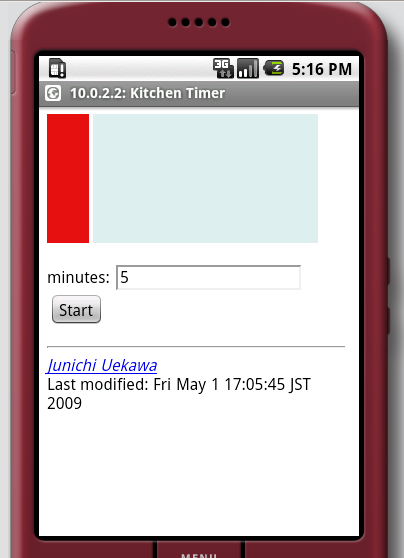
\includegraphics[width=0.3\hsize]{image200905/android-timer.png}

\subsection{Androidの簡単なアプリケーションを作成して起動してみる}

それでは、Android 用の簡単なアプリケーションを書いてみましょう。

\url{http://developer.android.com/guide/developing/eclipse-adt.html}
にしたがって淡々と作成します。
まず、
FileのNew Project で Android のをプロジェクト選択して作成しました。
ターゲットビルドは1.1にとりあえずしろと書いてありますが、よくわからない
ので、手元のファームウェアのバージョン 1.5 にあわせておきました。

RunのRun(Ctrl-F11)でAndroid Applicationを選択するとエミュレータを起動し
てアプリケーションを実行することができます。
最初に生成されたソースコードのままの状態だと Hello World アプリケーショ
ンが起動します。

\subsection{Androidの簡単なアプリケーションを書いてみる}

アプリケーションの作成やエディタの起動の部分はなんとかなるようになったの
で、次はチュートリアルを眺めてみます。
Hello Worldあたりがよさげです。

\url{http://developer.android.com/guide/tutorials/hello-world.html}

一通り読んで、とりあえずサンプルを眺めてどうやれば文字列を表示できるのか
を確認したので、好きな文字列を表示するアプリケーションを作ってみます。

Android の top コマンドでプロセスの一覧を出力できるので、
コマンドを実行してその出力を表示するだけのアプリケーションを作成してみま
した。
中核をなすsrc/jp.gr.netfort.dancer/TopView.javaは以下のようになりました。

\begin{commandline}
package jp.gr.netfort.dancer;

import android.app.Activity;
import android.os.Bundle;
import android.widget.TextView;
import java.io.*;

public class TopView extends Activity {
	/** Called when the activity is first created. */
	@Override
	public void onCreate(Bundle savedInstanceState) {
		super.onCreate(savedInstanceState);
		setContentView(R.layout.main);
		String [] command = { "top", "-n", "1"};
		String output = "";

		Runtime runtime = Runtime.getRuntime();
		Process process = null;
		try { 
			process = runtime.exec(command);
		} catch (Exception exception){
			System.exit(1);
		}
		BufferedReader reader = new BufferedReader(new InputStreamReader(process.getInputStream()));
		String line;
		try {
			while((line = reader.readLine()) != null) {
				output = output + line + "\n";
			}
		} catch (Exception exception) {
			System.exit(1);
		} finally {
			try {
				reader.close();
			} catch (Exception exception) {
				System.exit(1);
			}
		}
		TextView tv = new TextView(this);
		tv.setText(output);
		setContentView(tv);
	}
} 
\end{commandline}

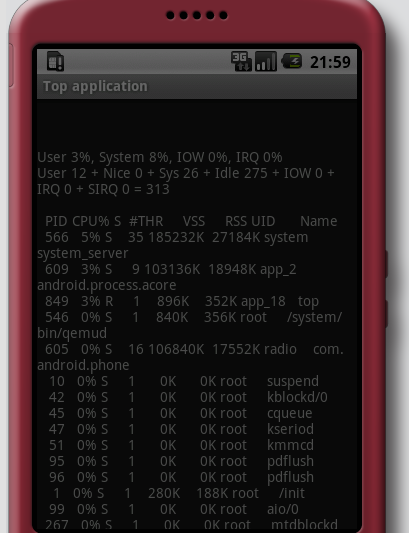
\includegraphics[width=0.3\hsize]{image200905/android-top.png}

\subsection{Androidの簡単なアプリケーションを実機で稼働させてみる}

実際に使う便利なアプリケーションを作ってみましょう。
ライトニングトークを実施する際にどのプレゼンテーションが気に入ったかを表
明する、投票用に利用するボタンでも作成しましょうか。

\subsubsection{エフェクト用のデータ}

まず、なんらかの効果音が必要です。
以前作成したding.wav をひろってきます。
res/raw 以下に nautilus からドラッグアンドドロップでコピーします。

あと、ボタン風味の画像が必要です。
適当にgimpで絵をかいて png ファイルを作成しました。

nautilus から res/drawable 以下に png ファイルをドラッグアンドドロップで
コピーします。

ファイル名からそのままリソースの名前を作成するため、-は利用できないよう
です、 \_ は利用できるようです。最初 he-up.png を作成しようとして、エラー
が出たので he\_up.png に変更しました。

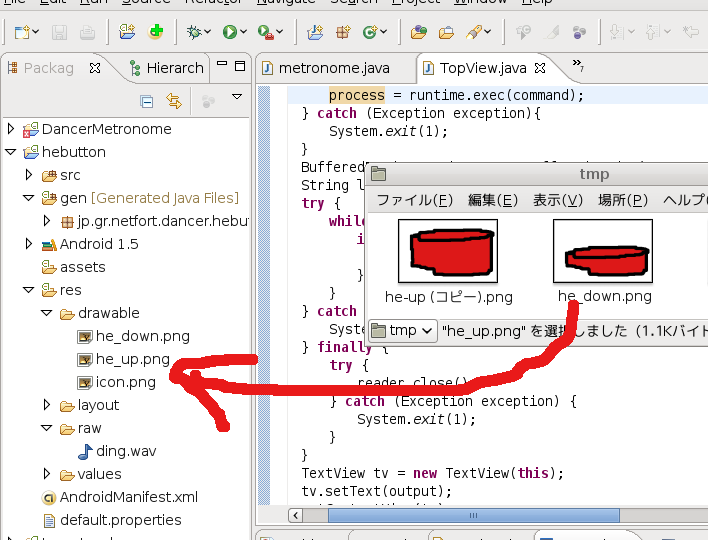
\includegraphics[width=0.5\hsize]{image200905/dragdrop.png}

\subsubsection{レイアウトの作成}

おもむろに ImageButton を作成して、srcに画像リソースを追加しておきましょ
う。

\subsubsection{クリックアクションの作成}

R.id.ImageButton01に対して onClickListenerを作成し、クリックされた瞬間の
反応を作成しましょう。

画像をクリックされた状態に切り替えるにはImageButtonのsetImageResource()
を呼び出せばよいようです。

音を出すには、MediaPlayer のインスタンスを作成し、start()を呼び出せばよ
いようです。

一定時間経過してから元の画像に戻すには、アラームを設定してコールバックし
てもらえるようにして、コールバックを呼び出されたときに処理をするようにす
ればよいようです。

\subsubsection{サーバ側のアクション}

それでは、クリックされたときにどういうことを行うのかのアクションを作成し
てみましょう。HTTPサーバを準備します。こういうイロモノ系のサーバを作成す
るときにはupaccho2 サーバを使うことが上川家の常識なので、それを踏襲しま
す。(予定)

\subsection{おまけ:開発環境に必要なメモリ消費は節減できるのか?}

手元のMacBookには1GBしかメモリを搭載していないです。
eclipse はデフォルトの設定だと起動した瞬間に1GB近くの
仮想メモリを消費し、即Swapを使用してしまうという問題がありました。

\begin{commandline}
  PID USER      PR  NI  VIRT  RES  SHR S %CPU %MEM    TIME+  COMMAND            
17124 dancer    20   0  972m 302m  20m S    1 31.2   0:39.85 java
\end{commandline}

とりあえず、ヒントを求めてmapsあたりを眺めてみます。
それなりにたくさんmmapしていますが、それだけでは説明できないようなメモリ
領域を確保しています。
\begin{commandline}
$ cat /proc/17124/status | grep Vm
VmPeak:	 1056748 kB
VmSize:	 1003316 kB
VmLck:	       0 kB
VmHWM:	  310740 kB
VmRSS:	  221616 kB
VmData:	  788504 kB
VmStk:	      84 kB
VmExe:	      36 kB
VmLib:	   38812 kB
VmPTE:	    1108 kB
$ cat /proc/17124/maps | grep rw | sort -rn -k5 
 .
\end{commandline}

とりあえずJavaのアプリケーションのHeapの使い方がよくわからないので、
jconsole で接続して問題を解析します。

メモリプールがいくつかあることがわかります。

\begin{itemize}
 \item  Tenured Gen が 60MB
 \item  Survivor 1MB
 \item  Code Cache が 4MB
 \item  Perm Gen が 70-90MB
 \item  Heapは100MB(GCしたら50MB程度)
\end{itemize}

eclipse.iniが現状こうなっているのですが、これをおそるおそるチューニングしてみます。
\begin{commandline}
-showsplash
org.eclipse.platform
-framework
plugins/org.eclipse.osgi_3.4.2.R34x_v20080826-1230.jar
-vmargs
-Dosgi.requiredJavaVersion=1.5
-Xms40m
-Xmx256m
-XX:MaxPermSize=256m
\end{commandline}

起動時に確保したヒープメモリの領域を開放していない部分については、GCを頻
繁に行えば起動は若干遅くなりますがうまくいけるような気がします。
Xmx 128mに変更してみると、若干メモリの消費が下がりました。
しかしそこまで劇的ではありませんね。
MaxPermSizeを64MBにするとエラー
\begin{commandline}
 Exception in thread "RMI TCP Connection(idle)" java.lang.OutOfMemoryError: PermGen space
\end{commandline}
が発生しました。
96MBだとエラーでおちないようです。

\begin{commandline}
  PID USER      PR  NI  VIRT  RES  SHR S %CPU %MEM    TIME+  コメント
17124 dancer    20   0  972m 302m  20m S    1 31.2   0:39.85 java
19663 dancer    20   0  795m 296m  23m S    1 30.6   0:36.69 Heap 128MB版
20266 dancer    20   0  661m 292m  22m S    1 30.1   0:41.62 MaxPermSize 96MB               
\end{commandline}

がんばってみた割にはメモリが10MB程度しか節約できませんでした。エミュレー
タも起動していると500MBくらいswapにいってしまうので、つらいです。しかも、
ギリギリのメモリ設定にしていたところ、いろいろと操作しているとメモリが足
りないというエラーで落ちました。こりゃダメだ。メモリ買いにいくかな。

\begin{commandline}
-showsplash
org.eclipse.platform
-framework
plugins/org.eclipse.osgi_3.4.2.R34x_v20080826-1230.jar
-vmargs
-Dosgi.requiredJavaVersion=1.5
-Xms40m
-Xmx128m
-XX:MaxPermSize=96m
\end{commandline}

\subsection{参考文献}

本記事の作成に参考にした文献です。

\begin{itemize}
 \item \url{http://www.eclipse.org/}: eclipse
 \item \url{http://developer.android.com/}: Android のページ、開発情報が
       まとまっている。特に\url{http://developer.android.com/sdk/1.5_r1/index.html}: Android
       SDK 1.5のダウンロードページからたどるページが重要。
 \item
      \url{http://developer.android.com/guide/basics/what-is-android.html}: 
      SDKの開発マニュアル。
      SDK の\url{./android-sdk-linux_x86-1.5_r1/docs/}に同じものがあるの
      でオフラインでも安心。
      ただしオンラインのドキュメントは微妙な訂正がアップデートされ続けて
      いるようなのでネットワーク接続が利用できるオンラインの場合はそちら
      を参照するほうがよいかもしれません。
\end{itemize}

% ===============================================================
\dancersection{DDTSS活用}{上川 純一}
\index{DDTSS}
\index{DDTP}
% ===============================================================

\subsection{はじめに}

最近 apt の国際化も進み、Debian archive のDescriptionの翻訳もパッケージ
の配布の仕組みと一緒に配布されるようになってきました。
一方、翻訳を用意するプロジェクト(DDTP:Debian Description Translation
Project)はまだ普及していません。
今回はその活用を事前課題として、今後どうやってうまく活用していくのかを考
えます。

\subsection{Debianのパッケージ説明文の翻訳の目的とは}

Debian Distributionには数万のパッケージがあります。
パッケージの説明文はインストールするソフトウェアを探すのに寄与する内容である必要があります。

現在、その説明文はすべて英
語で提供されています。
しかし、英語で記述されているとそもそも英語を理解していないとわからない部
分があり、しかも技術的な専門用語をまじえた説明文章は日本語を主言語とする
ユーザにとって理解しにくい場合があります。

そもそものDescriptionが翻訳に適するレベルに至っていない、日本語に訳しにく
い文章であれば、もとの文書を訂正するように依頼しましょう。

また、翻訳したDescriptionが日本語として理解しにくい、技術的な表現が不適切な表現であれば、その
Descriptionは適切ではないでしょう。

また、Debian全体で表記をできるだけ統一しましょう。同じ内容を説明するのに
表記のゆれがあるとパッケージの説明文をみているときにその差異に目がいって
しまいます。

その他に考慮する点は?

\subsection{DDTP}

DDTP の説明は Debian.org のページにあります: 
\url{http://www.debian.org/intl/l10n/ddtp.ja.html}。
\url{http://www.debian.or.jp/community/translate/description-ja.html}
などとあわせて眺めてください。

メールフロントエンドや、ウェブフロントエンドなどがあります。

\subsection{DDTSSとは}

DDTPのフロントエンドの一つがDDTSSです。
\url{http://ddtp.debian.net/ddtss/index.cgi/xx}
に提供されています。

\subsection{DDTSS活用の手順}

\subsubsection{アカウントの登録}

ログイン画面\footnote{\url{https://ddtp.debian.net/ddtss/index.cgi/login}}に飛ぶと、
アカウントを作成するためのリンク(Create 
Login\footnote{\url{https://ddtp.debian.net/ddtss/index.cgi/createlogin}})
があるので、そこからアカウント登録します。

メールが届くので、そこからリンクをクリックしてアカウントをアクティベート
すると、ログイン画面からログインできるようになります。

\subsubsection{パッケージ説明文の翻訳作成}

\url{http://ddtp.debian.net/ddtss/index.cgi/ja}画面で、
Pending Translation の欄にあるパッケージを適当にクリックすると、パッケー
ジ説明文の編集画面が登場します。
一部の文書が翻訳されておらず\verb!<trans>!となっていたり、まったく翻訳さ
れていなかったり、
状態はまちまちです。

この画面で翻訳を作成します。

\subsubsection{レビューの実施}

\url{http://ddtp.debian.net/ddtss/index.cgi/ja}画面で、
Pending Review の欄にあるパッケージを適当にクリックすると、パッケージ説
明文のレビュー画面が登場します。

レビューして変な部分があれば訂正しましょう。

\subsubsection{debian-docメーリングリストでのレビュー実施}

debian-docというメーリングリストで議論とかレビューはおこなうみたいです。

\subsection{参考文献}

以下のページも参考にしてください。

\begin{itemize}
 \item Debian パッケージの説明文を日本語で読みたい! 〜DDTP へのお誘い〜 
       \url{http://www.debian.or.jp/community/translate/description-ja.html}
 \item 武藤健志さんのblogの『Debianドキュメント翻訳手続き』:
       \url{http://kmuto.jp/d/index.cgi/debian/debian-doc-procedure.htm}
 \item 小林儀匡さんのDebian勉強会2006年9月資料「翻訳への誘い」:
       \url{tokyodebian.alioth.debian.org/pdf/debianmeetingresume200609.pdf}
 \item debian-doc メーリングリスト:
       主要な議論が行われています。質問なども、こちらで。
\end{itemize}


\clearpage

%\printindex

\cleartooddpage

\vspace*{15cm}
\hrule
\vspace{2mm}

\includegraphics[width=2cm]{image200502/openlogo-nd.eps}
\noindent \Large \bf Debian 勉強会資料\\ \\
\noindent \normalfont \debmtgyear{}年\debmtgmonth{}月\debmtgdate{}日 \hspace{5mm}  初版第1刷発行\\
\noindent \normalfont 東京エリア Debian 勉強会 (編集・印刷・発行)\\
\hrule


\end{document}
